\documentclass[margin=3mm]{standalone}
\usepackage{tikz}
\usetikzlibrary{shapes, arrows}

\tikzstyle{startstop} = [rectangle, rounded corners, minimum width=2cm, minimum height=1cm, text centered, draw=black, text=white, fill=black!80]
\tikzstyle{statement} = [rectangle, minimum width=4cm, minimum height=1cm, text centered, draw=black, fill=blue!20]
\tikzstyle{decision} = [rectangle, minimum height=1cm, text centered, draw=black, fill=yellow!30]
\tikzstyle{edge} = [thick, ->, >=stealth]

\begin{document}
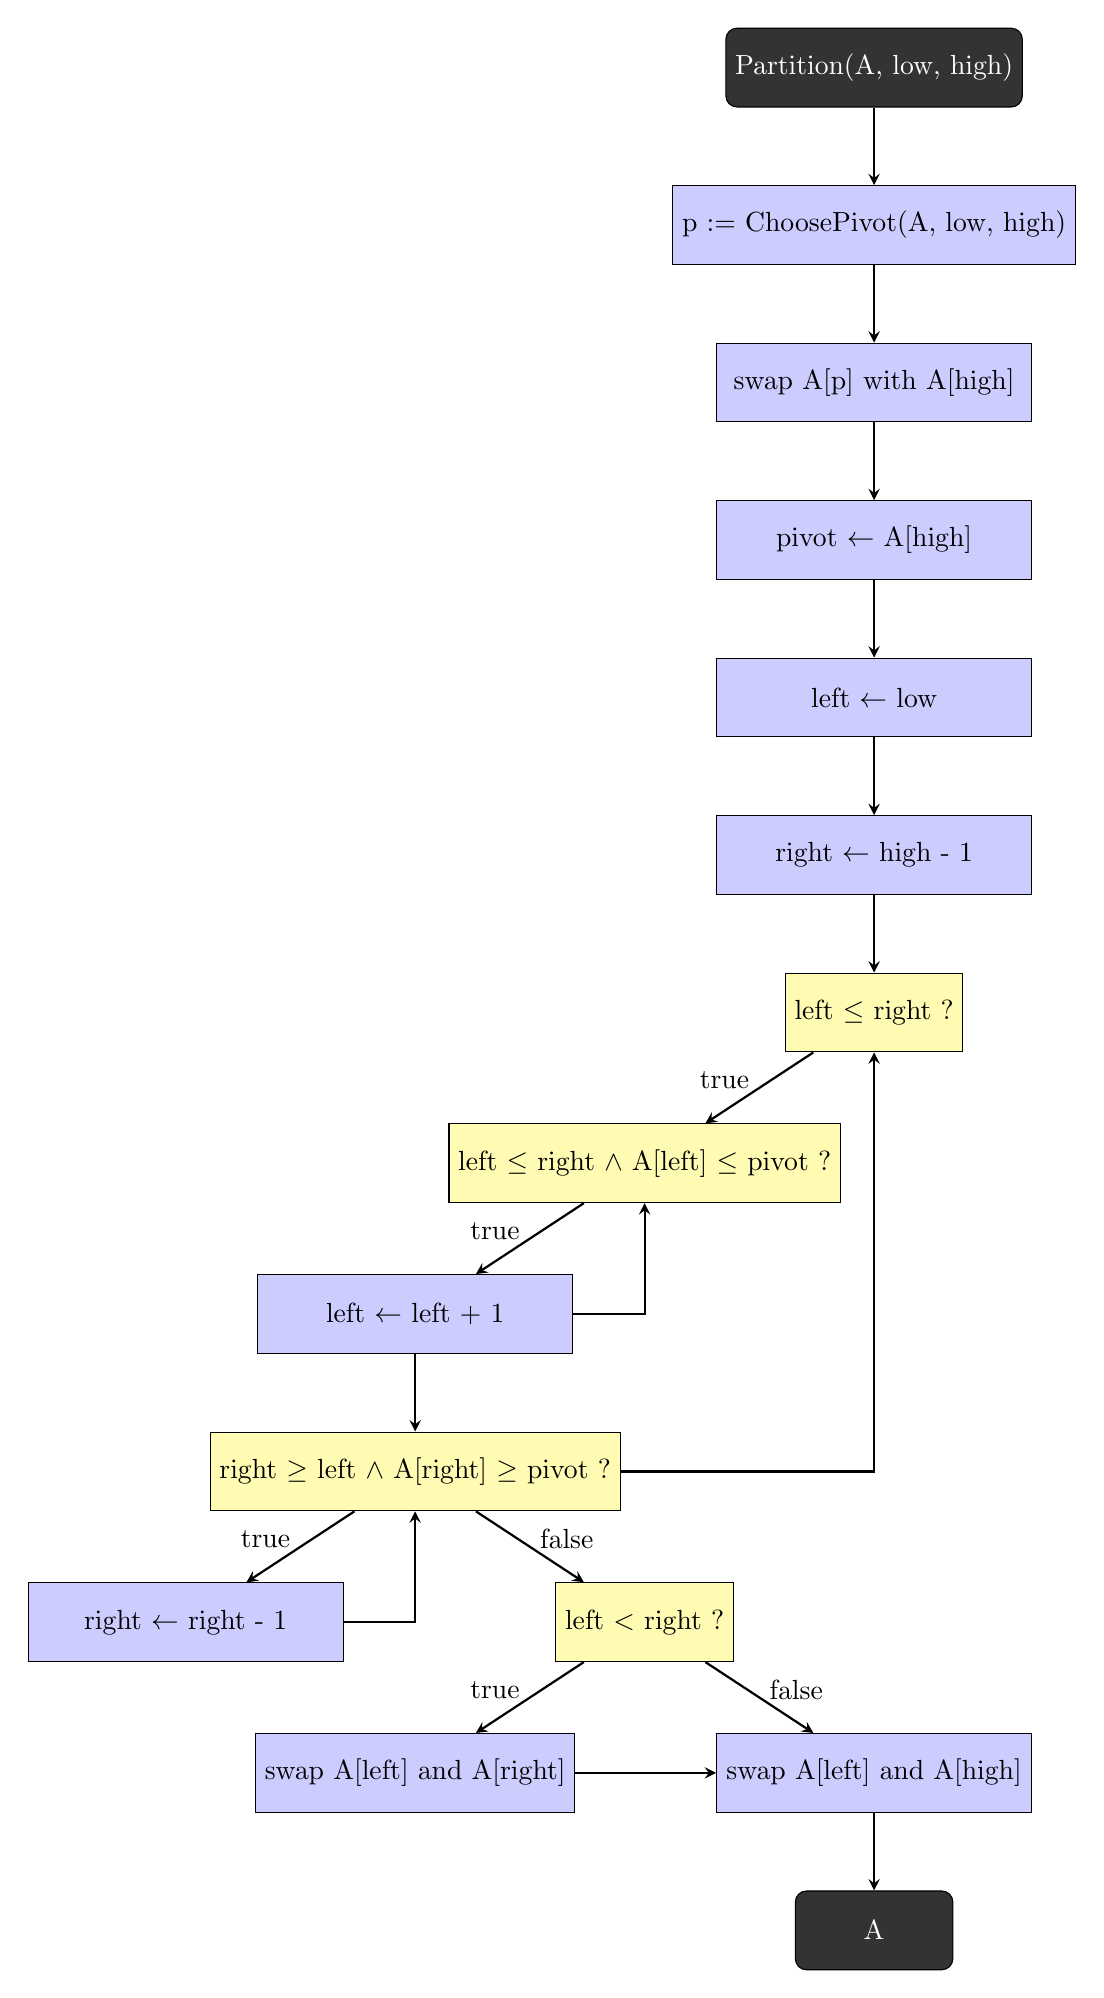
\begin{tikzpicture}[node distance=2cm]

\node (0) [startstop] {Partition(A, low, high)};
\node (1) [statement, below of=0] {p := ChoosePivot(A, low, high)};
\node (2) [statement, below of=1] {swap A[p] with A[high]};
\node (3) [statement, below of=2] {pivot $\gets$ A[high]};
\node (4) [statement, below of=3] {left $\gets$ low};
\node (5) [statement, below of=4] {right $\gets$ high - 1};
\node (6) [decision, below of=5] {left $\leq$ right ?};
\node (7) [decision, yshift=-0.5cm, xshift=-1.5cm, below left of=6] {left $\leq$ right $\land$ A[left] $\leq$ pivot ?};
\node (8) [statement, yshift=-0.5cm, xshift=-1.5cm, below left of=7] {left $\gets$ left + 1};
\node (9) [decision, below of=8] {right $\geq$ left $\land$ A[right] $\geq$ pivot ?};
\node (10) [statement, yshift=-0.5cm, xshift=-1.5cm, below left of=9] {right $\gets$ right - 1};
\node (11) [decision, yshift=-0.5cm, xshift=1.5cm, below right of=9] {left $<$ right ?};
\node (12) [statement, yshift=-0.5cm, xshift=-1.5cm, below left of=11] {swap A[left] and A[right]};
\node (13) [statement, yshift=-0.5cm, xshift=1.5cm, below right of=11] {swap A[left] and A[high]};
\node (14) [startstop, below of=13] {A};

\draw [edge] (0) -- (1);
\draw [edge] (1) -- (2);
\draw [edge] (2) -- (3);
\draw [edge] (3) -- (4);
\draw [edge] (4) -- (5);
\draw [edge] (5) -- (6);
\draw [edge] (6) -- node[anchor=east, yshift=0.1cm]{true} (7);
\draw [edge] (7) -- node[anchor=east, yshift=0.1cm]{true} (8);
\draw [edge] (8) -- (9);
\draw [edge] (8) -| (7);
\draw [edge] (9) -| (6);
\draw [edge] (9) -- node[anchor=west, yshift=0.1cm]{false} (11);
\draw [edge] (9) -- node[anchor=east, yshift=0.1cm]{true} (10);
\draw [edge] (10) -| (9);
\draw [edge] (11) -- node[anchor=west, yshift=0.1cm]{false} (13);
\draw [edge] (11) -- node[anchor=east, yshift=0.1cm]{true} (12);
\draw [edge] (12) -- (13);
\draw [edge] (13) -- (14);

\end{tikzpicture}
\end{document}